\documentclass[specification,annotation,times]{itmo-student-thesis}

%% Опции пакета:
%% - specification - если есть, генерируется задание, иначе не генерируется
%% - annotation - если есть, генерируется аннотация, иначе не генерируется
%% - times - делает все шрифтом Times New Roman, собирается с помощью xelatex
%% - pscyr - делает все шрифтом Times New Roman, требует пакета pscyr.

%% Делает запятую в формулах более интеллектуальной, например:
%% $1,5x$ будет читаться как полтора икса, а не один запятая пять иксов.
%% Однако если написать $1, 5x$, то все будет как прежде.
\usepackage{icomma}

%% Один из пакетов, позволяющий делать таблицы на всю ширину текста.
\usepackage{tabularx}

%% Данные пакеты необязательны к использованию в бакалаврских/магистерских
%% Они нужны для иллюстративных целей
%% Начало
\usepackage{tikz}
\usetikzlibrary{arrows}
\usepackage{filecontents}
\usepackage[demo]{graphicx}
\usepackage{caption}
\usepackage{subcaption}
\begin{filecontents}{master-thesis.bib}
@inproceedings{mason2009financial,
  title={Financial incentives and the performance of crowds},
  author={Mason, Winter and Watts, Duncan J},
  booktitle={Proceedings of the ACM SIGKDD workshop on human computation},
  pages={77--85},
  year={2009},
  organization={ACM},
  langid={english}
}

@article{lou2017use,
  title={Use of ontology structure and Bayesian models to aid the crowdsourcing of ICD-11 sanctioning rules},
  author={Lou, Yun and Tu, Samson W and Nyulas, Csongor and Tudorache, Tania and Chalmers, Robert JG and Musen, Mark A},
  journal={Journal of biomedical informatics},
  volume={68},
  pages={20--34},
  year={2017},
  publisher={Elsevier},
  langid={english}
}

@article{zhang2017consensus,
  title={Consensus algorithms for biased labeling in crowdsourcing},
  author={Zhang, Jing and Sheng, Victor S and Li, Qianmu and Wu, Jian and Wu, Xindong},
  journal={Information Sciences},
  volume={382},
  pages={254--273},
  year={2017},
  publisher={Elsevier},
  langid={english}
}

@article{allahbakhsh2013quality,
  title={Quality control in crowdsourcing systems: Issues and directions},
  author={Allahbakhsh, Mohammad and Benatallah, Boualem and Ignjatovic, Aleksandar and Motahari-Nezhad, Hamid Reza and Bertino, Elisa and Dustdar, Schahram},
  journal={IEEE Internet Computing},
  volume={17},
  number={2},
  pages={76--81},
  year={2013},
  publisher={IEEE},
  langid={english}
}

@article{lee2017crowdk,
  title={CrowdK: Answering top-k queries with crowdsourcing},
  author={Lee, Jongwuk and Lee, Dongwon and Hwang, Seung-won},
  journal={Information Sciences},
  volume={399},
  pages={98--120},
  year={2017},
  publisher={Elsevier},
  langid={english}
}

@article{raykar2010learning,
  title={Learning from crowds},
  author={Raykar, Vikas C and Yu, Shipeng and Zhao, Linda H and Valadez, Gerardo Hermosillo and Florin, Charles and Bogoni, Luca and Moy, Linda},
  journal={Journal of Machine Learning Research},
  volume={11},
  number={Apr},
  pages={1297--1322},
  year={2010},
  langid={english}
}

@inproceedings{demartini2012zencrowd,
  title={ZenCrowd: leveraging probabilistic reasoning and crowdsourcing techniques for large-scale entity linking},
  author={Demartini, Gianluca and Difallah, Djellel Eddine and Cudr{\'e}-Mauroux, Philippe},
  booktitle={Proceedings of the 21st international conference on World Wide Web},
  pages={469--478},
  year={2012},
  organization={ACM},
  langid={english}
}

@inproceedings{sheng2008get,
  title={Get another label? improving data quality and data mining using multiple, noisy labelers},
  author={Sheng, Victor S and Provost, Foster and Ipeirotis, Panagiotis G},
  booktitle={Proceedings of the 14th ACM SIGKDD international conference on Knowledge discovery and data mining},
  pages={614--622},
  year={2008},
  organization={ACM},
  langid={english}
}

@article{dang2015crowdsourcing,
  title={A crowdsourcing worker quality evaluation algorithm on MapReduce for big data applications},
  author={Dang, Depeng and Liu, Ying and Zhang, Xiaoran and Huang, Shihang},
  journal={IEEE Transactions on Parallel and Distributed Systems},
  volume={27},
  number={7},
  pages={1879--1888},
  year={2015},
  publisher={IEEE},
  langid={english}
}

@article{zhang2017consensus,
  title={Consensus algorithms for biased labeling in crowdsourcing},
  author={Zhang, Jing and Sheng, Victor S and Li, Qianmu and Wu, Jian and Wu, Xindong},
  journal={Information Sciences},
  volume={382},
  pages={254--273},
  year={2017},
  publisher={Elsevier},
  langid={english}
}

@article{nicholson2016label,
  title={Label noise correction and application in crowdsourcing},
  author={Nicholson, Bryce and Sheng, Victor S and Zhang, Jing},
  journal={Expert Systems with Applications},
  volume={66},
  pages={149--162},
  year={2016},
  publisher={Elsevier},
  langid={english}
}

@inproceedings{hung2013evaluation,
  title={An evaluation of aggregation techniques in crowdsourcing},
  author={Hung, Nguyen Quoc Viet and Tam, Nguyen Thanh and Tran, Lam Ngoc and Aberer, Karl},
  booktitle={International Conference on Web Information Systems Engineering},
  pages={1--15},
  year={2013},
  organization={Springer},
  langid={english}
}

@article{kara2015modeling,
  title={Modeling annotator behaviors for crowd labeling},
  author={Kara, Yunus Emre and Genc, Gaye and Aran, Oya and Akarun, Lale},
  journal={Neurocomputing},
  volume={160},
  pages={141--156},
  year={2015},
  publisher={Elsevier},
  langid={english}
}

@article{kuncheva2003limits,
  title={Limits on the majority vote accuracy in classifier fusion},
  author={Kuncheva, Ludmila I and Whitaker, Christopher J and Shipp, Catherine A and Duin, Robert PW},
  journal={Pattern Analysis \& Applications},
  volume={6},
  number={1},
  pages={22--31},
  year={2003},
  publisher={Springer},
  langid={english}
}

@inproceedings{khattak2011quality,
  title={Quality control of crowd labeling through expert evaluation},
  author={Khattak, Faiza Khan and Salleb-Aouissi, Ansaf},
  booktitle={Proceedings of the NIPS 2nd Workshop on Computational Social Science and the Wisdom of Crowds},
  volume={2},
  pages={5},
  year={2011},
  langid={english}
}

@inproceedings{lee2010social,
  title={The social honeypot project: protecting online communities from spammers},
  author={Lee, Kyumin and Caverlee, James and Webb, Steve},
  booktitle={Proceedings of the 19th international conference on World wide web},
  pages={1139--1140},
  year={2010},
  organization={ACM},
  langid={english}
}

@article{burmania2015increasing,
  title={Increasing the reliability of crowdsourcing evaluations using online quality assessment},
  author={Burmania, Alec and Parthasarathy, Srinivas and Busso, Carlos},
  journal={IEEE Transactions on Affective Computing},
  volume={7},
  number={4},
  pages={374--388},
  year={2015},
  publisher={IEEE},
  langid={english}
}

@article{li2016noise,
  title={Noise filtering to improve data and model quality for crowdsourcing},
  author={Li, Chaoqun and Sheng, Victor S and Jiang, Liangxiao and Li, Hongwei},
  journal={Knowledge-Based Systems},
  volume={107},
  pages={96--103},
  year={2016},
  publisher={Elsevier},
  langid={english}
}

@article{moon1996expectation,
  title={The expectation-maximization algorithm},
  author={Moon, Todd K},
  journal={IEEE Signal processing magazine},
  volume={13},
  number={6},
  pages={47--60},
  year={1996},
  publisher={IEEE},
  langid={english}
}

@article{dawid1979maximum,
  title={Maximum likelihood estimation of observer error-rates using the EM algorithm},
  author={Dawid, Alexander Philip and Skene, Allan M},
  journal={Journal of the Royal Statistical Society: Series C (Applied Statistics)},
  volume={28},
  number={1},
  pages={20--28},
  year={1979},
  publisher={Wiley Online Library},
  langid={english}
}

@inproceedings{whitehill2009whose,
  title={Whose vote should count more: Optimal integration of labels from labelers of unknown expertise},
  author={Whitehill, Jacob and Wu, Ting-fan and Bergsma, Jacob and Movellan, Javier R and Ruvolo, Paul L},
  booktitle={Advances in neural information processing systems},
  pages={2035--2043},
  year={2009},
  langid={english}
}

@inproceedings{raykar2009supervised,
  title={Supervised learning from multiple experts: whom to trust when everyone lies a bit},
  author={Raykar, Vikas C and Yu, Shipeng and Zhao, Linda H and Jerebko, Anna and Florin, Charles and Valadez, Gerardo Hermosillo and Bogoni, Luca and Moy, Linda},
  booktitle={Proceedings of the 26th Annual international conference on machine learning},
  pages={889--896},
  year={2009},
  organization={ACM},
  langid={english}
}

@inproceedings{karger2011iterative,
  title={Iterative learning for reliable crowdsourcing systems},
  author={Karger, David R and Oh, Sewoong and Shah, Devavrat},
  booktitle={Advances in neural information processing systems},
  pages={1953--1961},
  year={2011},
  langid={english}
}

@article{morris2012priming,
  title={Priming for better performance in microtask crowdsourcing environments},
  author={Morris, Robert R and Dontcheva, Mira and Gerber, Elizabeth M},
  journal={IEEE Internet Computing},
  volume={16},
  number={5},
  pages={13--19},
  year={2012},
  publisher={IEEE},
  langid={english}
}
\end{filecontents}

%% Указываем файл с библиографией.
\addbibresource{master-thesis.bib}

\begin{document}

\studygroup{M4238}
\title{Методы повышения эффективности процесса краудсорсинга с сохранением его воспроизводимости}
\author{Катунина Евгения Артёмовна}{Катунина Е. А.}
\supervisor{Фильченков Андрей Александрович}{Фильченков А.А.}{к.ф.-м.н.}{доц. кафедры КТ}
\publishyear{2019}
%% Дата выдачи задания. Можно не указывать, тогда надо будет заполнить от руки.
\startdate{01}{сентября}{2017}
%% Срок сдачи студентом работы. Можно не указывать, тогда надо будет заполнить от руки.
\finishdate{6}{мая}{2019}
%% Дата защиты. Можно не указывать, тогда надо будет заполнить от руки.
\defencedate{11}{июня}{2019}

\secretary{Павлова О.Н.}

%% Задание
%%% Техническое задание и исходные данные к работе
\technicalspec{Требуется усовершенствовать агрегацию ответов в краудсорсинге, добавив поведенческие признаки исполнителей (например, время ответа на вопрос, пропуск вопроса, возвращение к вопросу, количество смен ответа) в модель машинного обучения, и предсказать достоверность полученных от пользователей ответов. Модифицировать алгоритм Дэвида-Скина с помощью полученных значений. }

%%% Содержание выпускной квалификационной работы (перечень подлежащих разработке вопросов)
\plannedcontents{\begin{enumerate}
    \item Обзор предметной области;
    \item теоретические исследования;
    \item экспериментальная проверка методов решения и их сравнение.
\end{enumerate}}

%%% Исходные материалы и пособия 
\plannedsources{\begin{enumerate}
    \item Hung, Nguyen Quoc Viet, et al. "An evaluation of aggregation techniques in crowdsourcing." International Conference on Web Information Systems Engineering. Springer, Berlin, Heidelberg, 2013;
    \item Allahbakhsh, Mohammad, et al. "Quality control in crowdsourcing systems: Issues and directions." IEEE Internet Computing 17.2 (2013): 76-81;
    \item Aker, Ahmet, et al. "Assessing Crowdsourcing Quality through Objective Tasks." LREC. 2012.
\end{enumerate}}

%%% Цель исследования
\researchaim{Разработка метода повышения эффективности краудсорсинга.}

%%% Задачи, решаемые в ВКР
\researchtargets{\begin{enumerate}
    \item обзор существующих решений;
    \item реализация своего решения, улучшающего имеющиеся результаты;
    \item проведение эксперимента для сравнения лучших существующих решений с полученным в ходе выполнения работы.
\end{enumerate}}

\addadvancedsoftware{Библиотека для построения графиков XChart}{Глава 3}
\addadvancedsoftware{Библиотека для парсинга Univocity Parsers}{Глава 3}

%%% Использование современных пакетов компьютерных программ и технологий
%\addadvancedsoftware{Пакет \texttt{tabularx} для чуть более продвинутых таблиц}{\ref{sec:tables}, Приложения~\ref{sec:app:1}, \ref{sec:app:2}}
%\addadvancedsoftware{Пакет \texttt{biblatex} и программное средство \texttt{biber}}{Список использованных источников}%

%%% Краткая характеристика полученных результатов 
\researchsummary{Обучив модель машинного обучения случайный лес на данных с собранной статистикой о поведении пользователей, удалось улучшить качество широкоиспользующегося в краудсорсинговых платформах алгоритма Дэвида-Скина на 2\%, а также метод голосования большинства на 1.7\% с помощью добавления информации о поведении пользователей. Результаты работы могут быть применены в краудсорсинговых платформах.}

%%% Гранты, полученные при выполнении работы 
\researchfunding{Отсутствуют.}

%%% Наличие публикаций и выступлений на конференциях по теме выпускной работы
\researchpublications{
\begin{refsection}
Публикации:

1. Катунина Е. А. Методы повышения качества краудсорсинга // Сборник тезисов докладов конгресса молодых ученых. Электронное издание. 2019.

Конференции:

1. VIII Конгресс молодых учёных, 2019 г., тема доклада: Методы повышения качества краудсорсинга.

\end{refsection}
}

%% Эта команда генерирует титульный лист и аннотацию.
\maketitle{Магистр}

%% Оглавление
\tableofcontents

%% Макрос для введения. Совместим со старым стилевиком.
\startprefacepage

Крадсорсинг -- это метод решения задач с помощью коллективного разума путём разбиения одной большой сложной задачи на много маленьких простых подзадач, выдачи этих подзадач Интернет-пользователям для получения их решений и последующей агрегации полученных от Интернет-пользователей ответов. В настоящее время краудсорсинг активно используется IT-компаниями для сбора обучающих наборов данных для моделей машинного обучения, примерами решаемых с помощью краудсорсинга задач являются:
\begin{itemize}
    \item распознавание изображений;
    \item распознавание речи;
    \item ранжирование страниц поисковой выдачи;
    \item фильтрация спама, порнографии;
    \item обнаружение дубликатов и т.д.
\end{itemize}

Краудсорсинг за пятнадцать лет своего существования использовался не только для развития искусственного интеллекта, примеры других задач, которые пытались решать с помощью краудсорсинга:
\begin{itemize}
    \item поиски пропавших людей по фотографиям со спутников (краудсорсинг не помог в решении этого типа задач);
    \item помощь дизайнерам (люди выбирают, какой подход к оформлению чего-либо им больше нравится);
    \item различные опросы;
    \item NASA размещает фотографии с космического телескопа и анализирует снимки, на которых исполнители находят интересные объекты;
    \item полевые задания, выполняемые на местности, например, обновление информации в мобильных картах о часах работы заведений и т.д.
\end{itemize}

Для размещения заданий и сбора ответов используются краудсорсинговые платформы, например Яндекс.Толока, Amazon Mechanical Turk, Crowdflower, Microworkers. На данных платформах можно зарегистрироваться как <<заказчик>> и размещать задания, либо как <<исполнитель>> для выполнения заданий.

Существует множество факторов, влияющих на качество ответов, получаемых с помощью краудсорсинга, среди них можно выделить такие факторы:
\begin{enumerate}
    \item плохая формулировка задач заказчиком;
    \item неудачно подобранный заказчиком размер поощрения за выполнение задач;
    \item недобросовестность исполнителей;
    \item человеческий фактор (применимо к исполнителям).
\end{enumerate}

В плохую формулировку задач заказчиком входит:
\begin{enumerate}
    \item отсутствие примеров задач и их решения;
    \item расплывчатые формулировки задач;
    \item размер задачи (крупные задачи необходимо разбивать на подзадачи) и т.д.
\end{enumerate}

В исследовании ~\cite{allahbakhsh2013quality} сформулирована хорошая рекомендация к составлению заданий: честно ответить на задание не должно быть сложнее, чем выбрать ответ случайно, вопросы должны быть простыми и чёткими.

Согласно исследованию ~\cite{mason2009financial}, более значительные денежные поощрения по сравнению со стандартно использующимися заказчиками на данной краудсорсинговой платформе позволяют быстрее получить ответы от исполнителей, но качество может быть хуже, чем при умеренном размере денежных поощрений, в то же время слишком низкий размер поощрений также может отражаться на качестве полученных ответов.

Среди известных проблем краудсорсинга можно выделить проблему спама, например, в 2011 году доля спамеров среди исполнителей на платформе Amazon Mechanical Turk составляла целых 39\%. Краудсорсинговые платформы позволяют бороться со спамерами с помощью добавления контрольных вопросов, определения минимальной доли правильных ответов на них и недопуска исполнителей, у которых не получилось преодолеть минимальный порог доли правильных ответов, однако у такого подхода к борьбе со спамерами есть очевидные проблемы: вопросы могут быть слишком сложными, и добросовестные участники также могут не справиться с ними, не очевидно, какую долю правильных ответов нужно устанавливать в качестве минимальной. Также у краудсорсинговых платформ есть возможность автоматического отклонения ответов, которые даны исполнителями слишком быстро, либо заказчик может сам отклонить ответ на основе предоставленных ему данных о выполнении задания исполнителем.

Наконец, последний фактор, человеческий, применим к исполнителям, не являющимся спамерами, но желающим больше заработать и выполняющим задания, несмотря на усталость или сомнения в верности своих ответов.

У краудсорсинговых платформ существуют механизмы, позволяющие заказчику наказывать некомпетентных исполнителей: понижать их рейтинг в системе, отклонять их задания, вследствие чего они не получат за них никаких вознаграждений; можно изначально разрешать выполнять задания только исполнителям с определённым минимальным рейтингом или определённым минимальным уровнем экспертизы в данной области. У такого подхода имеются проблемы: заказчики тоже не всегда добросовестные, могут получить ответы от пользователей и отклонить их, чтобы не производить выплаты, также на ручной контроль качества заказчиком требуется его личное время, что не всегда приемлемо для заказчиков. 

Ещё одним способом контроля качества ответов является конвейерный подход, разделённый на следующие стадии:
\begin{enumerate}
    \item первая группа исполнителей отвечает на вопросы, сформулированные заказчиком;
    \item вторая группа получает эти вопросы и ответы на них и оценивает, верные ответы или нет;
    \item третья группа исполнителей проверяет, верно ли вторая группа оценила ответы первой группы.
\end{enumerate}
Если на втором или третьем этапе обнаружилась ошибка, задания выдаются заново другим исполнителям. Весь процесс продолжается, пока не будет достигнут определённый уровень согласованности ответов.

Идея данной выпускной квалификационной работы состоит в том, чтобы улучшить качество агрегации ответов следующим образом:
\begin{enumerate}
    \item анализировать поведение исполнителей программным образом, без непосредственного участия заказчика или других исполнителей, например, участник может долго отвечать на задание или наоборот слишком быстро, может много раз менять ответ, а может дать его сразу, может возвращаться к заданию и т.д.;
    \item на основе поведенческих признаков построить рейтинг пользователей со значениями уровня доверия к их ответам;
    \item модифицировать хорошо зарекомендовавший себя и использующийся во многих краудсорсинговых платформах алгоритм Дэвида-Скина, добавив туда информацию о поведении пользователей.
\end{enumerate}

В первой главе данной работы будет проведён обзор существующих методов контроля качества в краудсорсинге.

Во второй главе будут рассмотрены теоретические аспекты проведённого иследования: признаки для методов машинного обучения, метрика, с помощью которой можно оценить результат, способ модификации алгоритма Дэвида-Скина.

В третьей главе будет описан проведённый эксперимент, приведены детальные результаты, и будет выявлен наилучший из методов решения задачи.

%% Начало содержательной части.
\chapter{Обзор предметной области}

%% Так помечается начало обзора.
\startrelatedwork
%%Пример ссылок в рамках обзора: \cite{example-english, example-russian, unrestricted-jump-evco, nsga-ii-steady-state}.

%% Так помечается конец обзора.
%%Вне обзора:~\cite{bellman}.

%%\section{Таблицы}\label{sec:tables}
\section{Агрегация ответов}
Этапами краудсорсинга являются создание заданий, размещение их в системе, получение ответов пользователей (этап разметки), агрегация полученных от пользователей ответов. Последний этап является наиболее наукоёмким и будет рассматриваться в данном разделе.
\subsection{Постановка задачи}
Для того чтобы агрегировать ответы пользователей нужно решить задачу поиска консенсуса, которая формально описывается для краудсорсинга следующим образом \cite{zhang2017consensus}. $E=\{e_{i}\}_{i=1}^{I}$ - набор заданий, задание $e_{i}=(x_{i}, y_{i}),$ где $x_{i}$ -- набор значений признаков, $y_{i}$ -- истинная метка. $U=\{u_{j}\}_{j=1}^{J}$ -- множество пользователей. Метки принадлежат множеству классов $C=\{c_{k}\}_{j=1}^{K}$. В случае бинарной классификации, которая часто встречается среди задач краудсорсинга, класс $c_{1}$ $(k=1)$ соответствует положительным меткам, а класс $c_{2}$ $(k=2)$ -- отрицательным. Всем заданиям $i$ сопоставлено множество меток $l_{i}=\{l_{ij}\}_{j=1}^{J}$, где элемент $l_{ij}$ получен от участника $j$. $L=\{l_{i}\}_{i=1}^{I}$ -- матрица аннотаций, где $l_{ij}\in \{c_{1},0,c_{2}\}$, 0 означает, что участник  не отвечал на данное задание. Участник $j$ описывается матрицей $N^{(j)}=\{n_{ik}^{j}\},1\leq i\leq I,1\leq k\leq K,$ здесь каждый элемент равен количеству раз, когда пользователь $j$ отнёс пример из задания $i$ к классу $k$. Обычно $n_{ik}^{j}$ равно нулю или единице. Также для всех классов известны априорные вероятности.

Задачи состоит в подборе таких меток $\hat{y_{i}}$, на которых достигается минимальное значение функции ошибки:
\[R=\frac{1}{I}\sum_{i=1}^{I}\mathbf{I}(\hat{y_{i}} \neq y_{i})\] 
при заданных $L$ и $y\in (c_{1}, c_{2})$, где $\mathbf{I}$ -- индикаторная функция.

\section{Методы агрегации ответов}
Методы агрегации ответов можно разделить на итеративные и неитеративные \cite{hung2013evaluation}. Неитеративные методы используют эвристики для вычисления агрегированного значения для каждого вопроса по отдельности. Итеративные методы представляют серию итераций. На каждой итерации выполняется два шага обновлений:
\begin{enumerate}
    \item обновление агрегированных значений для каждого вопроса, основанные на оценке исполнителей;
    \item корректировка оценки для каждого исполнителя, основанная на ответах, данных им.
\end{enumerate}

Преимуществами неитеративных методов являются простота реализации и быстрое время выполнения, преимущество итеративных методов -- лучшее качество агрегации ответов по сравнению с неитеративными методами.

\subsection{Неитеративные методы агрегации ответов}
Простейшим неитеративным методом агрегации ответов является голосование большинства (Majority Decision, MD) \cite{kuncheva2003limits}: правильный ответ тот, за который проголосовало больше всего пользователей. Однако в данной модели все пользователи вносят равный вклад в итоговый ответ, что является существенной проблемой.

Метод Honeypot (HP) \cite{lee2010social} является улучшением голосования большинства за счёт добавления контрольных вопросов. Однако у данного метода тоже есть проблема: хотя контрольные вопросы и позволяют избавиться от спамеров, добросовестные исполнители тоже могут быть неверно идентифицированы как спамеры, если контрольные вопросы слишком сложные.

Метод ELICE (Expert Label Injected Crowd Estimation) \cite{khattak2011quality} является улучшением Honeypot: добавляется минимальная доля правильных ответов исполнителя на контрольные вопросы, необходимая, чтобы приступить к заданию, также сложность контрольных вопросов оценивается по тому, насколько люди справляются с ними.

\subsection{Итеративные методы агрегации ответов}
Итеративные методы основаны на EM-алгоритме \cite{moon1996expectation}, позволяющем найти оценку максимального правдоподобия вероятностных моделей. Алгоритмы, основанные на методе EM, характерны тем, что сначала даётся начальная оценка правильных ответов на задания, затем оптимизируются параметры, эти действия повторяются, пока не будет достигнута определённая сходимость или не будет выполнено максимальное число итераций, то есть данные алгоритмы работают схожим образом и отличаются лишь набором параметров. Например, в методе Дэвида-Скина \cite{dawid1979maximum} параметром модели является матрица ошибок участников, в GLAD \cite{whitehill2009whose} -- степени компетентности участников и сложности заданий, в SLME \cite{raykar2009supervised} используются чувствительность и специфичность. Итеративный метод ITER \cite{karger2011iterative} отличается от остальных тем, что для каждого ответа исполнителя представлена его надёжность, уровень исполнителя оценивается как сумма значений надёжности, взвешенная по сложности вопросов, другие методы представляют надёжность ответов исполнителя как одно число.

\subsection{Результаты сравнения итеративных и неитеративных методов}
В работе \cite{hung2013evaluation} описывается сравнение итеративных и неитеративных методов агрегации ответов с помощью фреймворка, созданного авторами, симулирующего разные типы исполнителей (эксперты, обычные, малоопытные, однообразные спамеры (дают один и тот же ответ), случайные спамеры, разные типы вопросов (два варианта ответа или больше). При сравнении методов учитывались такие метрики как время вычислений, точность, устойчивость к спамерам, адаптивность к мультиразметке. Выводы, которые можно сделать из результатов сравнения, таковы:
\begin{itemize}
    \item В целом, EM и SLME достигают наибольшей точности и надёжно работают против спамеров. В частности, они превосходят другие методы, когда число ответов на вопросы велико.
    \item Если среди исполнителей много спамеров (от 30 \%), лучше использовать SLME или EM. Интересно, что производительность неитеративных методов (MD, HP, ELICE) не значительно меньше SLME и EM. Если высокая точность не требуется, они лучше всего подходят для приложений, требующих быстрых вычислений. Наиболее чувствительны к спамерам GLAD и ITER.
    \item Только MD, HP, EM могут адаптироваться к мультиразметке. Для двоичной разметки, EM – победитель. В случае четырёх меток MD и HP также подходящие варианты, разница между ними и EM минимальна.
    \item Для приложений, требующих быстрых вычислений, MD и HP – победители. Напротив, строго не рекомендуется использовать итеративные методы. Время вычислений не только намного больше, чем у неитеративных методов, но и приходится заново вычислять все агрегированные ответы с приходом новых ответов исполнителей.
\end{itemize}

\section{Классические алгоритмы агрегации ответов}
В данном разделе будут рассмотрены алгоритмы, которые сейчас применяются в большинстве краудсорсинговых платформ, и являются наиболее известными в своём роде.

\subsection{Алгоритм Дэвида-Скина}
Наиболее популярным и часто использующимся в краудсорсинговых платформах является алгоритм Дэвида-Скина. Алгоритм Дэвида-Скина решает задачу поиска консенсуса, описанную вначале главы, следующим образом: для каждого пользователя $j$ имеется матрицей ошибок классификации $\pi^{(j)}_{kl}$, которая задаёт вероятность, что пользователь $j$ выберет класс $l$ для задания, истинный класс которого $k$. На expectation-шаге по матрице ответов пользователей $L$ алгоритм вычисляет вероятности того, что пример $i$ является объектом класса $k$ (для каждого класса) в соответствии со следующим уравнением:
\[P(\hat{y}_{i}=c_{k}|L)=\frac{\prod_{j=1}^{J}\prod_{l=1}^{L}(\pi^{(j)}_{kl})^{n_{il}^{j}}P(c_{k})}{\sum_{q=1}^{K}\prod_{j=1}^{J}\prod_{l=1}^{L}(\pi^{(j)}_{ql})^{n_{il}^{j}}P(c_{q})}\]
, где $P(c_{k})$ и $P(c_{q})$ -- априорные вероятности того, что пример относится к классам $c_{k}$ и $c_{q}$ соответственно, вычисленные на maximization-шаге алгоритма. На maximization-шаге уточняются значения матрицы ошибок классификации:
\[\hat{\pi}_{kl}^{(j)}=\frac{\sum_{i=1}^{I}I(\hat{y_{i}}=c_{k})n_{il}^{(j)}}{\sum_{l=1}^{K}\sum_{i=1}^{I}I(\hat{y_{i}}=c_{k})n_{il}^{(j)}},\]
Также на maximization-шаге уточняются априорные вероятности классов:
\[\hat{P}(c_{k})=\frac{1}{I}\sum_{i=1}^{I}I(\hat{y_{i}}=c_{k}).\]

Истинные классы примеров неизвестны, поэтому вместо $I(\hat{y_{i}}=c_{k})$ используется математическое ожидание этой величины: $P(\hat{y_{i}}=c_{k}|L).$

Начальное приближение для правильных ответов обычно выбирается с помощью простого голоса большинства, для матрицы ошибок изначально считается, что пользователи идеальны и не допускали ошибок при ответе на вопросы. 

\subsection{Алгоритм GLAD}
GLAD моделирует уровень компетентности каждого пользователя $(\alpha_{j}\in(-\infty, +\infty))$ и сложность каждого задания $(\frac{1}{\beta_{i}}\in [0,+\infty))$. Чтобы оценить уровень компетентности пользователя $j$ для задания $i$ используется следующая логистическая модель:
\[P(l_{ij}=y_{i}|\alpha_{j},\beta_{i})=\frac{1}{1+e^{-\alpha_{j}\beta_{i}}}.\]

На expectation-шаге алгоритм вычисляет апостериорные вероятности для положительных и отрицательных классов для всех примеров по значениям параметров $(\alpha, \beta)$ с последнего шага maximization и матрицы аннотаций $L$:
\[P(y_{i}=+|L,\alpha,\beta)=P(y_{i}=+|l_{i},\alpha,\beta_{i})\propto P(y_{i}=+)\prod_{j=1}^{J}p(l_{ij}|y_{i}=+,\alpha_{j},\beta_{i}).\]

На maximization-шаге алгоритм максимизирует стандартную функцию $Q$ и обновляет значения двух параметров $(\alpha, \beta)$, используя алгоритм градиентного спуска следующим образом:
\[Q(\alpha,\beta)=E[\ln P(L,y|\alpha,\beta)]=E[\ln\prod_{i=1}^{I}(P(y_{i}=+)\prod_{j=1}^{J}P(l_{ij}|y_{i}=+,\alpha_{j}, \beta_{i}))],\]
где $y$ содержит предполагаемые метки для всех заданий.

\subsection{Алгоритм Raykar, Yu (RY)}
Алгоритм RY \cite{raykar2010learning} моделирует чувствительность $(\alpha_{j})$ и специфичность $(\beta_{j})$ пользователя $j.$ В случае двоичных меток чувствительность определяет смещение (bias) в сторону положительного класса, а специфичность -- смещение в сторону отрицательного класса.

RY использует байесовский подход к оценке априорной вероятности параметров $(\alpha_{j},\beta_{j})$ и положительного класса:
\[P(\alpha_{j}|a_{j}^{+},a_{j}^{-})=Beta(\alpha_{j}|a_{j}^{+},a_{j}^{-}),\]

\[P(\beta_{j}|b_{j}^{+},b_{j}^{-})=Beta(\beta_{j}|b_{j}^{+},b_{j}^{-}),\]

\[P(p^{+}|n^{+},n^{-})=Beta(p^{+}|n^{+},n^{-}),\]
где $a_{j}^{}$
 и $a_{j}^{-}$ -- число положительных и отрицательных меток соответственно, выданных пользователем $j$ для положительного класса, рассматриваемого в данный момент; $b_{j}^{+}$ и $b_{j}^{-}$ -- число положительных и отрицательных меток соответственно, выданных пользователем $j$ для отрицательного класса, рассматриваемого в данный момент; $n^{+}$ и $n^{-}$ -- число положительных и отрицательных меток, соответственно, выданных всеми пользователями для всех примеров. $Beta$ -- это $\beta$-функция вероятностного распределения.

На expectation-шаге по примеру $x_{i}$, матрице аннотаций $L$, двум параметрам $(\alpha,\beta)$ и априорной вероятности положительного класса $p^{+}$ RY вычисляет вероятность принадлежности каждого примера $i$ к положительному классу:

\[\mu_{i}=P(y_{i}=+|x_{i},L,\alpha,\beta,p^{+})\propto\frac{p^{+}a_{i}}{p^{+}a_{i}+(1-p^{+})b_{i}},\]
где 
\[a_{i}=\prod_{j=1}^{J}(\alpha_{j})^{\mathbf{I}(L_{ij}=+)}(1-\alpha_{j})^{\mathbf{I}(L_{ij}=-)}\]
\[b_{i}=\prod_{j=1}^{J}(\beta_{j})^{\mathbf{I}(L_{ij}=-)}(1-\beta_{j})^{\mathbf{I}(L_{ij}=+)}.\]

На maximization-шаге RY обновляет параметры $(\alpha_{j},\beta_{j})$ пользователя $j$ и априорную вероятность положительного класса $p^{+}$ в соответствии с разметкой, проведённой пользователем $j$ $(\sum_{i=1}^{I}l_{ij})$:

\[\alpha_{j}=\frac{a_{j}^{+}-1+\sum_{i=1}^{I}\mu_{i}l_{ij}}{a_{j}^{+}+a_{j}^{-}-2-\sum_{i=1}^{I}\mu_{i}}\]
\[\beta_{j}=\frac{b_{j}^{+}-1+\sum_{i=1}^{I}(1-\mu_{i})(1-l_{ij})}{b_{j}^{+}-b_{j}^{-}-2+\sum_{i=1}^{I}(1-\mu_{i})}\]
\[p^{+}=n^{+}-1+\frac{\sum_{i=1}^{I}\mu_{i}}{n^{+}-n^{-}-2+I}.\]

\subsection{Алгоритм ZenCrowd}
ZenCrowd \cite{demartini2012zencrowd} использует только один двоичный параметр ${good, bad}$ для моделирования надёжности пользователя. Это сложнее, чем голосование большинства, но проще чем остальные описанные выше методы. Метод используется для решения задачи связывания сущностей для крупных коллекций веб-страниц.

На expectation-шаге по всей разметке от каждого пользователя $j$ $(\sum_{i=1}^{I}l_{ij})$ ZenCrowd вычисляет надёжность пользователя $j$:

\[P(u_{j}=reliable)=\frac{\sum_{i=1}^{I}\mathbf{I}(l_{ij}=y_{i})}{\sum_{k=1}^{K}\sum_{i=1}^{I}n_{ik}}.\]

На maximization-шаге ZenCrowd использует надёжности пользователей, чтобы обновить вероятность принадлежности примера $i$ классу $c_{k}$:
\[P(y_{i}=c_{k})=\frac{\prod_{j=1}^{J}[P(u_{j}=reliable)]^{\mathbf{I}(y_{i}=c_{k})}}{\sum_{k=1}^{K}\prod_{k=1}^{w}[P(u_{j}=reliable)]^{\mathbf{I}(y_{i}=c_{k})}}.\]

\section{Последние исследования в области агрегации ответов}
Ранее были рассмотрены классические методы агрегации ответов, которые используются уже давно. Последние исследования в этой области связаны с тем, что классические алгоритмы всё же не очень хорошо справляются со смещённой оценкой пользователей (например, в заданиях, где нужно определить, содержит ли видео элементы порнографии, люди, у которых есть дети, чаще относят примеры к содержащим порнографию), а также они не учитывают человеческий фактор (усталость и потерю концентрации).

В работе \cite{sheng2008get} авторы модифицируют алгоритм Дэвида-Скина, смещая метку, которую поставил пользователь, к истинной, и утверждают, что им удалось улучшить результаты. В статье \cite{zhang2017consensus} авторы утверждают, что взвешенный голос большинства, в котором в качестве весов используются оценки смещения по частоте положительных и отрицательных меток от пользователей, в целом, имеет лучшую производительность, чем все четыре классических алгоритма, описанные выше и основанные на Expectation-Maximization алгоритме.

В работе \cite{burmania2015increasing} авторы добавляют проверочные задания с известным результатом во время разметки заданий пользователем, чтобы определить момент, когда он устал, и прекратить выдачу ему заданий. В \cite{morris2012priming} описано использование техники прайминга (фиксирования установки), пользователям показывались определённые изображения или включались аудиозаписи, создающие определённое эмоциональное состояние, данный метод позволил улучшить полученные результаты. В статье \cite{lou2017use} упомянут такой способ улучшения качества краудсорсинга как добавление на страницу с заданием, ссылок, описывающих специфичные термины, однако не представлены результаты применения этого метода.

В работе \cite{lee2017crowdk} представлены методы отбора лучших вариантов из заданного набора. В работах \cite{nicholson2016label} и \cite{li2016noise} предлагаются методы очистки зашумлённых данных с помощью обученных классификаторов, то есть классификаторы также выступают в роли пользователей краудсорсинговых платформ, выполняющих задания. В статье \cite{dang2015crowdsourcing} используют map-reduce для больших данных и улучшают качество агрегации ответов. В исследовании \cite{kara2015modeling} авторы предлагают четыре новых модели, основанные на байесовских методах, и утверждают, что их модели дают лучшие результаты, чем широко применяющиеся сейчас.

\chapterconclusion
В главе 1 были рассмотрены разные типы алгоритмов агрегации ответов в краудсорсинге, было подробно рассмотрено четыре классических алгоритма, которые часто используются в современных краудсорсинговых платформах (особенно алгоритм Дэвида-Скина). Также были рассмотрены современные научные работы, в которых авторы предлагают новые методы и утверждают, что они работают лучше классических, а также предлагают способы улучшения качества с существующими алгоритмами, в том числе онлайн-решения, реализуемые ещё на этапе разметки.

\finishrelatedwork

\chapter{Теоретические аспекты исследования}

\section{Признаки для применения машинного обучения}
Были составлены следующие признаки, хорошо описывающие поведение пользователя:
\begin{enumerate}
    \item время ответа на вопрос;
    \item число смен ответа;
    \item число выбранных вариантов ответа;
    \item время между выбором окончательного ответа и его подтверждением;
    \item среднее время ответа для данного исполнителя;
    \item среднее время ответа для данного вопроса;
    \item время бездействия;
    \item время с начала сессии.
\end{enumerate}

Признак <<время ответа на вопрос>> в комбинации с признаками <<среднее время ответа для данного исполнителя>> и <<среднее время ответа для данного вопроса>> позволяет определить,  когда пользователь очень быстро отвечает, скорее всего, не подумав, или наоборот очень сомневается в ответе и отвечает слишком долго. Признак <<число смен ответа>> описывает сомнения пользователя при выборе ответа, учитывается наведение курсора то на один ответ, то на другой, выбор ответа, смена ответа на другой. Признак <<число выбранных вариантов>> ответа описывает сколько разных вариантов ответа попало под курсор или было выбрано. Среднее значение времени ответа для данного исполнителя позволяет оценивать насколько типичным для него является ответ на один вопрос за то или иное время. Среднее время ответа для данного вопроса позволяет оценить сложность вопроса. Время бездействия позволяет учитывать ситуацию, когда пользователь отвлёкся, например, ушёл пить кофе. Время с начала сессии позволяет оценить, насколько пользователь устал, а следовательно, упала его концентрация. Признак <<время между выбором окончательного ответа и его подтверждением>> описывает степень сомнения в ответе.

\section{Метод машинного обучения}

Предполагается использовать в качестве обучающего множества признаковое описание ответов пользователей ($F_{1}(x_{i}^{(j)})\dots F_{z}(x_{i}^{(j)})$, где $F_{z}$ -- функция, извлекающая признак под номером $z$, $x_{i}^{j}$ -- ответ пользователя под номером $j$ на задание с номером $i$), которому сопоставлены метки $y_{i}=1$, если ответ совпал с истинным, $y_{i}=0$ в противном случае, обучить <<случайный лес>> и получить для каждого ответа уверенность в том, что он правильный ($score_{i}^{(j)}$, значения $score_{i}^{j}$ вещественные от нуля до единицы), затем на основе этих данных вычислить оценку для каждого пользователя по среднему значению уверенности в его ответах ($user^{(j)}=\frac{\sum_{i=1}^{N}score_i^{j}}{N},$ гдe $N$ -- число заданий, на которые ответил пользователь, $user^{(j)}$ также принимает вещественные значения от нуля до единицы). 

Было решено использовать в качестве метода машинного обучения <<случайный лес>>, так как он традиционно показывает более хорошие результаты для задач регрессии, нежели остальные методы. Количество деревьев в случайном лесе -- 200, глубина деревьев не ограничена.

\subsection{Оценка качества модели машинного обучения}

Для оценки качества обучения будут использованы матрица ошибок классификации, точность, полнота и $F1$-мера отдельно для каждого класса и в среднем, бинарная логистическая функция потерь, квадратный корень из среднеквадратического отклонения между рассчитанными для пользователей значениями $user$ и долей правильных ответов пользователей по всем вопросам $q$, где для пользователя $j$ $q_{j} = \frac{\sum_{i=1}^{N}I(a_{u}^{i}, a_{c}^{i})}{N}$, где $a_{u}^{i}$ -- ответ пользователя $u$ на задание $i$, $a_{c}^{i}$ -- правильный ответ на задание $i$, $I$ -- возвращает 1, если аргументы равны, и 0, в противном случае.

Квадратный корень из среднеквадратической ошибки:
\[RMSE=\sqrt{\frac{\sum_{i=1}^{n}(y_{i} - \hat{y_{i}})^{2}}{n}}.\]

Бинарная логистическая функция потерь:
\[logloss=-\frac{1}{l}\cdot\sum_{i=1}^{l}(y_{i}\cdot\log(\hat{y_{i}}) + 
(1-y_{i})\cdot\log(1-\hat{y_{i}})),\] где $\hat{y}$ -- ответ алгоритма на $i$-м объекте, $y$ -- истинная метка класса на $i$-ом объекте, а $l$ - размер выборки.

\[F_{1}=2\cdot\frac{precision\cdot recall}{precision + recall}\], где $F_{1}$ - $F_{1}$-мера, $recall=\frac{TP}{TP+FN}$, $precision = \frac{TP}{TP+FP}$, $TP\ (True\ Positive)$ -- число верно классифицированных как положительные объектов, $FP\ (False\ Positive)$ -- число неверно класифицированных как положительные объектов, $FN\ (False\ Negative)$ -- число неверно класифицированных как отрицательные объектов, $TN\ (True\ Negative)$ -- число верно классифицированных как отрицательные объектов. $F_{1}$-мера, $precision$ и $recall$ оцениваются для каждого класса по отдельности, затем эти метрики качества классификации, рассчитанные для каждого класса по отдельности, суммируются и дают оценку качества классификации в целом.

Матрица ошибок классификации представлена в таблице \ref{confusionMatrix}.

\begin{table}[!h]
\caption{Матрица ошибок классификации}
\label{confusionMatrix}
\centering
\begin{tabularx}{\textwidth}{|*{18}{>{\centering\arraybackslash}X|}}\hline
-- & $y=1$ & $y=0$ \\\hline
$\hat{y}=1$ & TP  & FP  \\\hline
$\hat{y}=0$ & FN & TN \\\hline
\end{tabularx}
\end{table}

Для оценки важности признаков будет использоваться устройство случайного леса, чем выше узел с признаком в дереве, тем большую часть выборки он делит пополам, и, соответственно, вносит больший вклад в качество бинарной классификации.

\section{Рассматриваемые способы улучшения качества агрегации ответов}
В данном разделе будут рассмотрены модификации с добавлением информации о поведении пользователей для базового алгоритма, голосования большинства, и для одного из наиболее часто применяющихся при агрегации ответов в краудсорсинговых платформ алгоритма, алгоритма Дэвида-Скина. Будет рассмотрен способ скрещивания этих методов.

\subsection{Модификация алгоритма Дэвида-Скина}
Оригинальный алгоритм Дэвида-Скина вычисляет вероятности того, что пример $i$ является объектом класса $k$ (для каждого класса) в соответствии со следующим уравнением:
\[P(\hat{y}_{i}=c_{k}|L)=\frac{\prod_{j=1}^{J}\prod_{l=1}^{L}(\pi^{(j)}_{kl})^{n_{il}^{j}}P(c_{k})}{\sum_{q=1}^{K}\prod_{j=1}^{J}\prod_{l=1}^{L}(\pi^{(j)}_{ql})^{n_{il}^{j}}P(c_{q})}.\]
Добавим в это уравнение матрицу достоверности ответов $B$, учитывая, что $B$ не зависит от $L$:
\[P(\hat{y}_{i}=c_{k}|L, B)=\frac{\prod_{j=1}^{J}\prod_{l=1}^{L}(\pi^{(j)}_{kl}\cdot b_{ikl}^{(j)})^{n_{il}^{j}}P(c_{k})}{\sum_{q=1}^{K}\prod_{j=1}^{J}\prod_{l=1}^{L}(\pi^{(j)}_{ql}\cdot b_{iql}^{(j)})^{n_{il}^{j}}P(c_{q})},\]
где $b_{ikl}^{(j)} = score_{i}^{j}$ при $k=l$, иначе $b_{ikl}^{(j)} = 1 - score_{i}^{(j)}$.

В качестве второго варианта модификации рассмотрим следующее уравнение:
\[P(\hat{y}_{i}=c_{k}|L, U)=\frac{\prod_{j=1}^{J}\prod_{l=1}^{L}(\pi^{(j)}_{kl}\cdot u_{kl}^{j})^{n_{il}^{j}}P(c_{k})}{\sum_{q=1}^{K}\prod_{j=1}^{J}\prod_{l=1}^{L}(\pi^{(j)}_{ql}\cdot u_{ql}^{j})^{n_{il}^{j}}P(c_{q})},\]
где $U$ -- матрица доверия к пользователям, $u_{kl}^{(j)} = user^{j}$ при $k=l$, иначе $u_{kl}^{(j)} = 1 - user^{(j)}$.

\subsection{Взвешенный голос большинства}
В обычном голосовании большинства веса ответов равны, и никак не учитывается их достоверность. Можно получить агрегированные ответы по тому же принципу, что и в обычном голосовании большинства, но использовать в качестве весов предсказания нашей модели машинного обучения для каждого ответа.
\[y_{i}=argmax_{c\in[1,\dots,J]}(\sum_{j=1}^{K}w_{j}\mathbf{1}(y_{i}^{j}=c)),\]
где $y_{i}$ -- агрегированный ответ под номером $i$, $c$ -- метка класса, $J$ -- количество возможных меток, $K$ -- количество голосов, $w_{j}$ -- вес голоса $j$.

\subsection{Взвешенный голос большинства с добавлением матрицы ошибок Дэвида-Скина}
Можно попробовать улучшить результаты, добавив к исследуемым поведенческим признакам частоту ошибок из алгоритма Дэвида-Скина, которая для каждого пользователя оценивается как сумма недиагональных элементов матрицы ошибок классификации:
\[ER_{j}=\sum_{l=1}^{L}\sum_{k=1}^{L}(\pi^{(j)}_{kl}) - \sum_{k=1}^{L}(\pi^{(j)}_{kk}),\]
где $ER_{j}$ -- частота ошибок пользователя $j$.

\section{Метрики качества агрегации ответов}
Как правило, выходными данными алгоритма агрегации является помимо самих агрегированных ответов, уверенность в том, что они верные (от 0 до 1). Для оценки качества методов агрегации можно использовать бинарную логистическую функцию потерь:
\[Q=-\frac{1}{N}\cdot\sum_{i=1}^{N}(-y_{i}\log(p_{i})+(1-y_{i})\log(1-p_{i})),\]
где $Q$ -- качество агрегации, $N$ -- число заданий, $p_{i}$ -- вероятность того, что агрегированный ответ на задание $i$ верный, $y_{i}=0$, если агрегированный ответ на задание $i$ неверный и $y_{i}=1$ в противном случае. Чем ближе к нулю полученное значение, тем лучше.

Когда задачи простые, и в их решениях у отдельных пользователей не может быть разногласий, все агрегированные ответы могут получиться верными. В этом случае можно посчитать качество метода агрегации следующим образом:
\[Q=\frac{\sum_{i=1}^{n}p(a_{i})}{n},\]
где $Q$ -- качество агрегации, $n$ -- число заданий, $a_{i}$ -- агрегированный ответ для задания под номером $i$, $p$ -- вероятность того, что ответ верный. В данном случае, наоборот, чем ближе полученное значение к единице, тем лучше качество агрегации.

\chapterconclusion
Во второй главе были представлены поведенческие признаки, которые будут использоваться для построения модели оценки достоверности ответов пользователей с помощью метода машинного обучения <<случайный лес>>, хорошо зарекомендовавшего себя для решения задач регрессии и классификации, способы проверки качества обученной модели классификации и оценки важности признаков. Были рассмотрены способы модификации алгоритма Дэвида-Скина, широко использующегося в краудсорсинговых платформах и традиционно демонстрирующего хорошее качество агрегации ответов, также были рассмотрены способы улучшить простое голосование большинства взвешиванием с поведенческими признаками и добавлением такого признака как частота ошибок пользователей, полученного из модели Дэвида-Скина. Были рассмотрены метрики, которые позволят оценить качество агрегации ответов в случае, если все агрегированные ответы верны, и в случае, когда есть неверные ответы.

\chapter{Описание эксперимента и результатов}
\section{Описание набора данных}
Для проведения эксперимента был выбран набор данных <<Russe'2018: Human-Annotated Sense-Disambiguated Word Contexts for Russian>>. Этот набор данных содержит идентифицированные людьми значения слов для 2562 контекстов из 20 слов, используемых в задаче RUSSE'2018 по устранению неоднозначности в смыслах слов для русского языка. Помимо ответов пользователей в наборе данных присутствует статистика о поведении пользователей, отражены действия в UI и время для каждого из них. Исследование проводилось с помощью краудсорсинговой платформы Яндекс.Толока.

Пример задания: дан отрывок из текста \begin{displayquote}<<..., и провалов, к счастью, не было. Правда, в некоторых случаях наши рекламные акции могут закончиться судебным разбирательством. Но иногда бренду, для того чтобы себя эффективно...>>,\end{displayquote} нужно оценить значение слова <<акции>> в данном контексте, варианты ответов:
\begin{enumerate}
    \item <<ценная бумага, выпускаемая акционерным обществом>>;
    \item <<действие, выступление кого-либо, предпринимаемое для достижения какой-либо цели>>.
\end{enumerate}

\begin{figure}
  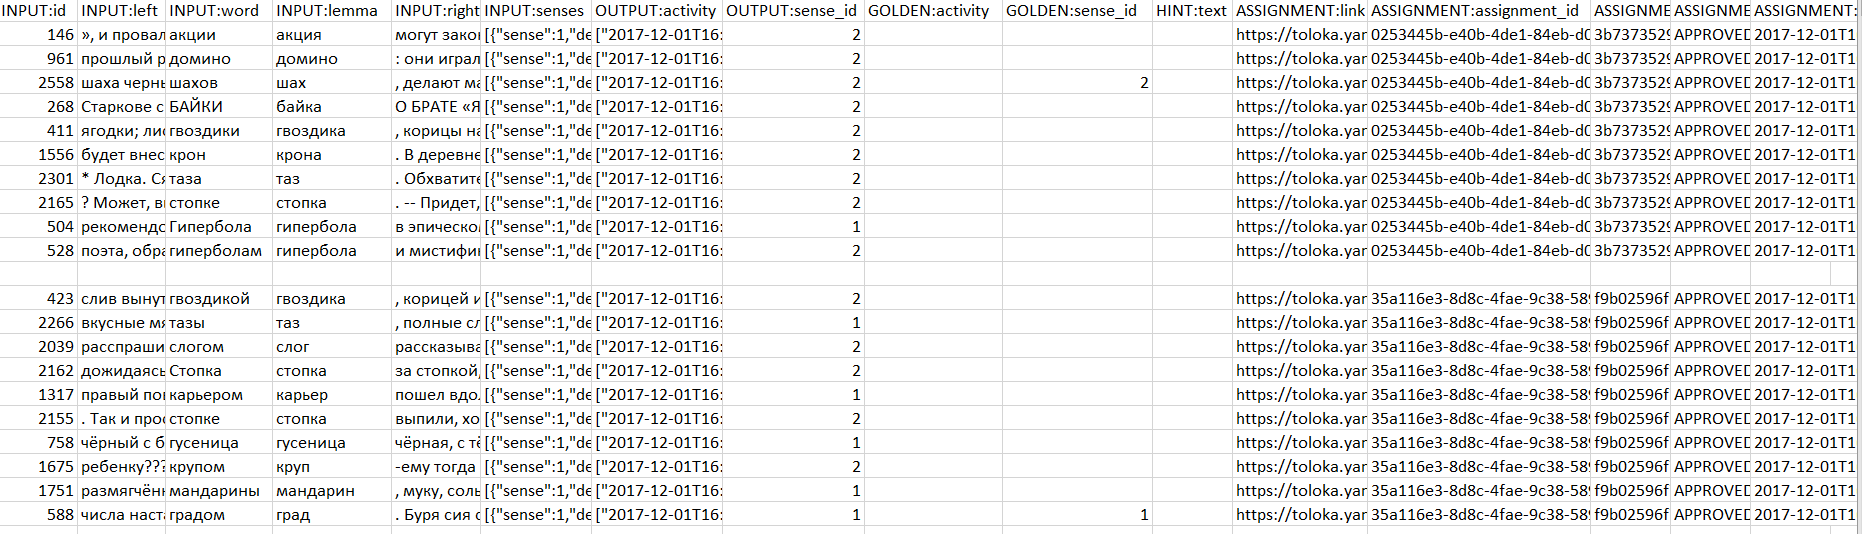
\includegraphics[width=\linewidth]{dataset1.PNG}
  \caption{Набор данных, часть 1}
  \label{fig:dataset1}
\end{figure}

\begin{figure}
  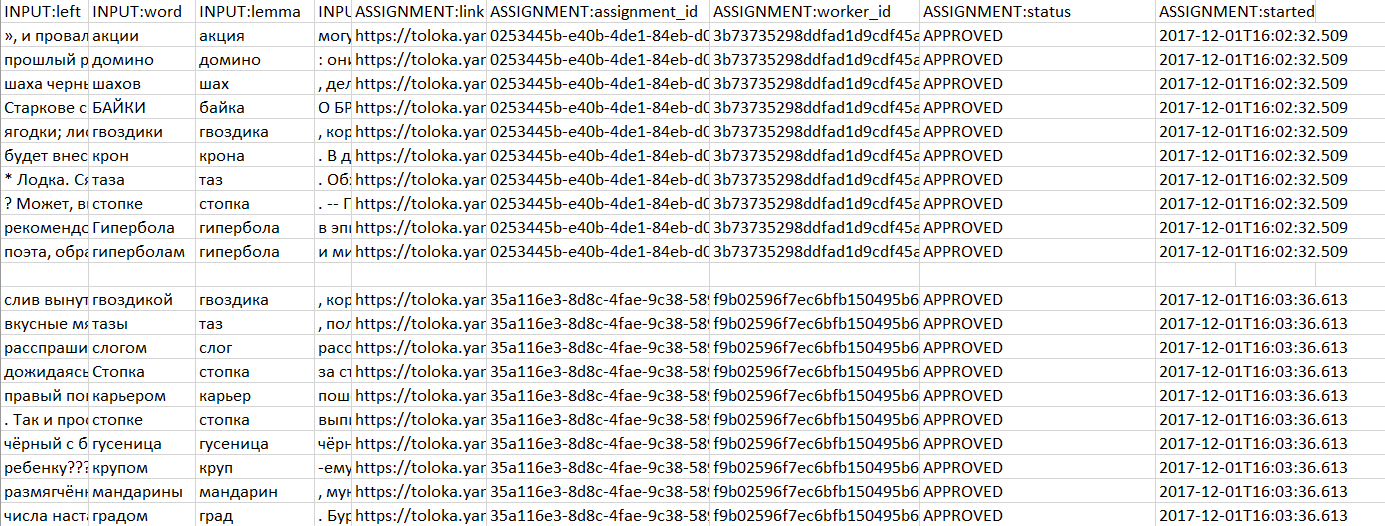
\includegraphics[width=\linewidth]{dataset2.PNG}
  \caption{Набор данных, часть 2}
  \label{fig:dataset2}
\end{figure}

На рисунках \ref{fig:dataset1} и \ref{fig:dataset2} представлена часть набора данных. Поля данных (слева направо):
\begin{itemize}
    \item <<INPUT:id>> -- номер задания;
    \item <<INPUT:left>> -- часть текста до слова, значение которого нужно оценить;
    \item <<INPUT:word>> -- слово, значение которого нужно оценить, в том падеже и числе, в котором оно употребляется в отрывке из текста;
    \item <<INPUT:lemma>> -- слово, значение которого нужно оценить в именительном падеже единственном числе;
    \item <<INPUT:right>> -- часть текста после слова, значение которого нужно оценить;
    \item <<INPUT:senses>> -- значения слова, из которых нужно выбрать;
    \item <<OUTPUT:activity>> -- взаимодействие пользователя c UI веб-страницы при ответе на вопрос, данные представлены в формате JSON;
    \item <<OUTPUT:sense\_id>> -- ответ, выбранный пользователем;
    \item <<GOLDEN:activity>> -- автоматически сгенерировалось Яндекс.Толокой, поле не имеет смысла и всегда пустое;
    \item <<GOLDEN:sense\_id>> -- если вопрос контрольный, правильный ответ, иначе поле пустое;
    \item <<HINT:text>> -- подсказок к заданиям не было, поэтому данное поле всегда пустое;
    \item <<ASSIGNMENT:link>> -- ссылка на страницу с заданиями;
    \item <<ASSIGNMENT:assignment:id>> -- идентификатор страницы с заданиями;
    \item <<ASSIGNMENT:worker\_id>> -- идентификатор пользователя;
    \item <<ASSIGNMENT:status>> -- статус задания, принято заказчиком или отклонено;
    \item <<ASSIGNMENT:started>> -- время и дата, когда отрендерилась страница с заданиями.
\end{itemize}

Все задания были приняты заказчиком (имели статус <<APPROVED>>). Заданий было 2562, пользователей 116, в среднем на пользователя приходилось по 83 задания. Гистограмма с распределением по количеству заданий на пользователя представлена на рисунке \ref{fig:tasks}. 

\begin{figure}
  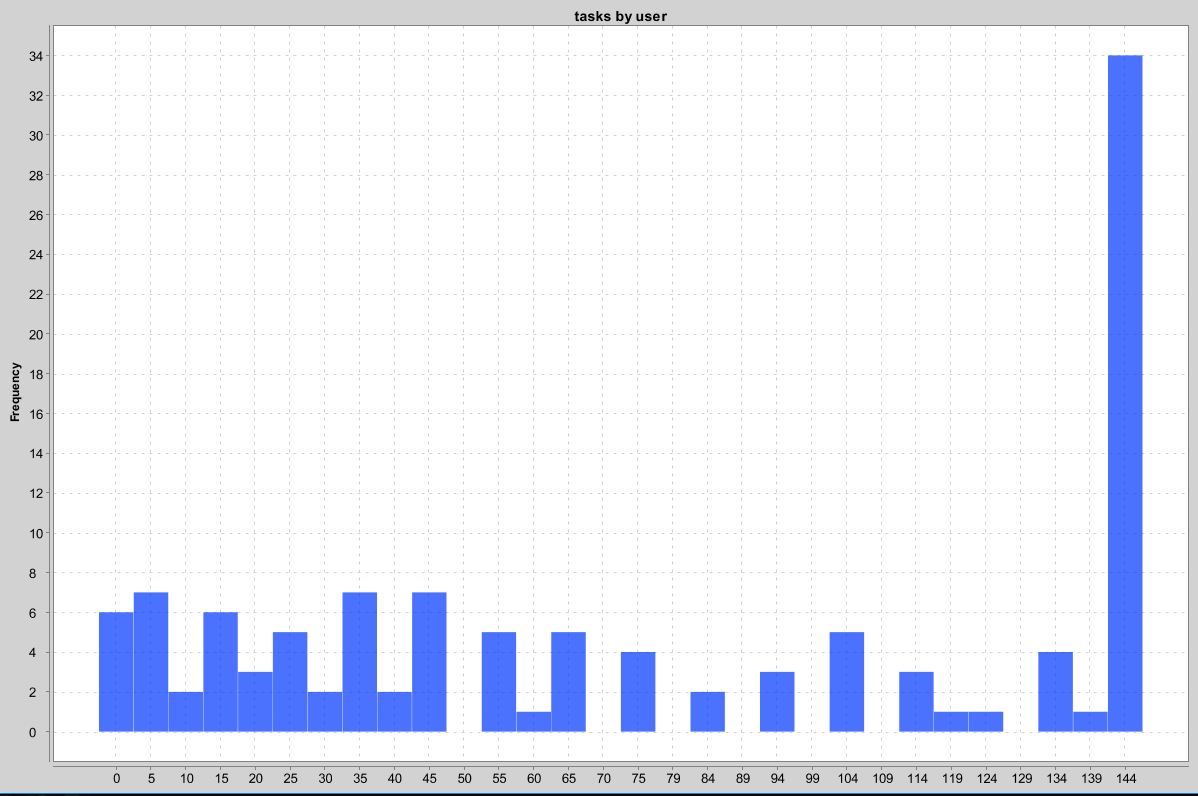
\includegraphics[scale=0.5]{tasks.PNG}
  \caption{Гистограмма числа заданий, выполненных пользователями}
  \label{fig:tasks}
\end{figure}

\section{Извлечение признаков}
Пример данных об активности пользователя при ответе на вопрос представлен на рисунке \ref{fig:activity}. Изначально JSON разбивался на список строк, содержащихся внутри квадратных скобок, то есть на отдельные действия в UI. Первое событие (страница с заданиями отрендерилась) никак не учитывалось. Время ответа на вопрос рассчитывалось как разница между временем для последнего действия и второго. Время после подтверждения ответа на вопрос рассчитывалось как разница между временем для последнего действия и действия <<click>>. Число смен ответа оценивалось по количеству действий <<mouseenter>>. Число вариантов ответа рассчитывалось по количеству разных значений у <<answer>>. Время бездействия оценивалось как сумма периодов времени, когда никаких действий в UI не происходило дольше 20 секунд.

Ответы, для которых по техническим причинам не было собрано достаточно данных об активности (была собрана не полностью, либо было только первое действие, отрисовка страницы) не учитывались и по ним не извлекались признаки.

На гистограммах \ref{fig:answer_changes}-\ref{fig:users_error_rate} представлены данные о распределении значений неотнормированных признаков (для подачи на вход алгоритму машинного обучения признаки нормировались от 0 до 1). В данные о некоторых признаках были внесены изменения, так как исходные данные портили нормировку признаков, были выбросы со слишком большими значениями, значения, принятые для выбросов, отмечены на подписях к рисункам. 

\begin{figure}
  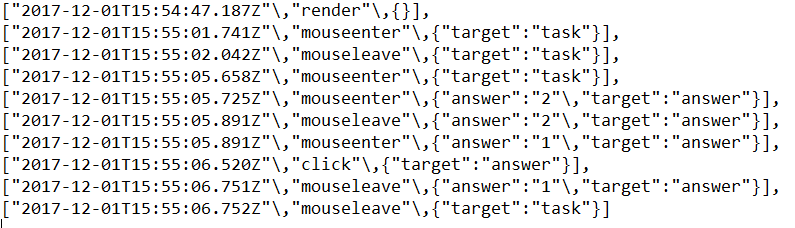
\includegraphics[scale=0.5]{activity.PNG}
  \caption{Пример данных об активности пользователя при ответе на вопрос}
  \label{fig:activity}
\end{figure}

\begin{figure}
  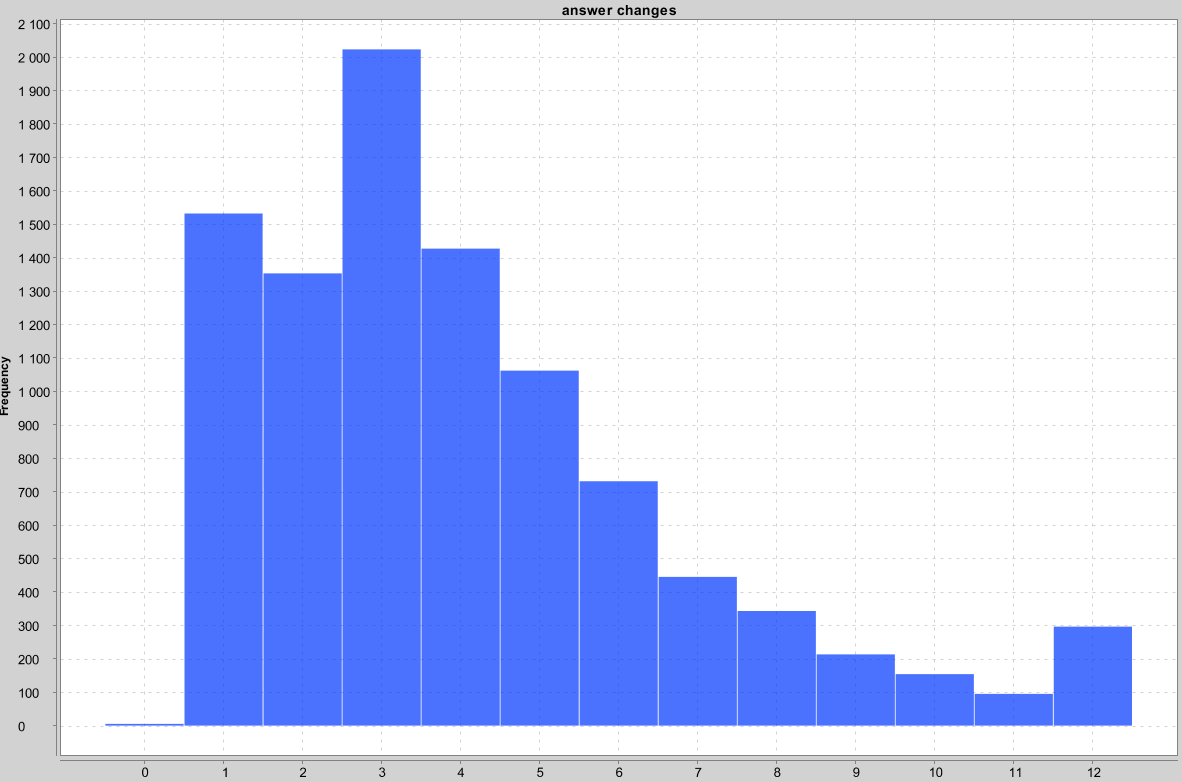
\includegraphics[scale=0.5]{answer_changes.PNG}
  \caption{Число смен ответа. Для выбросов, портящих нормировку признака, было принято значение 13.}
  \label{fig:answer_changes}
\end{figure}

\begin{figure}
  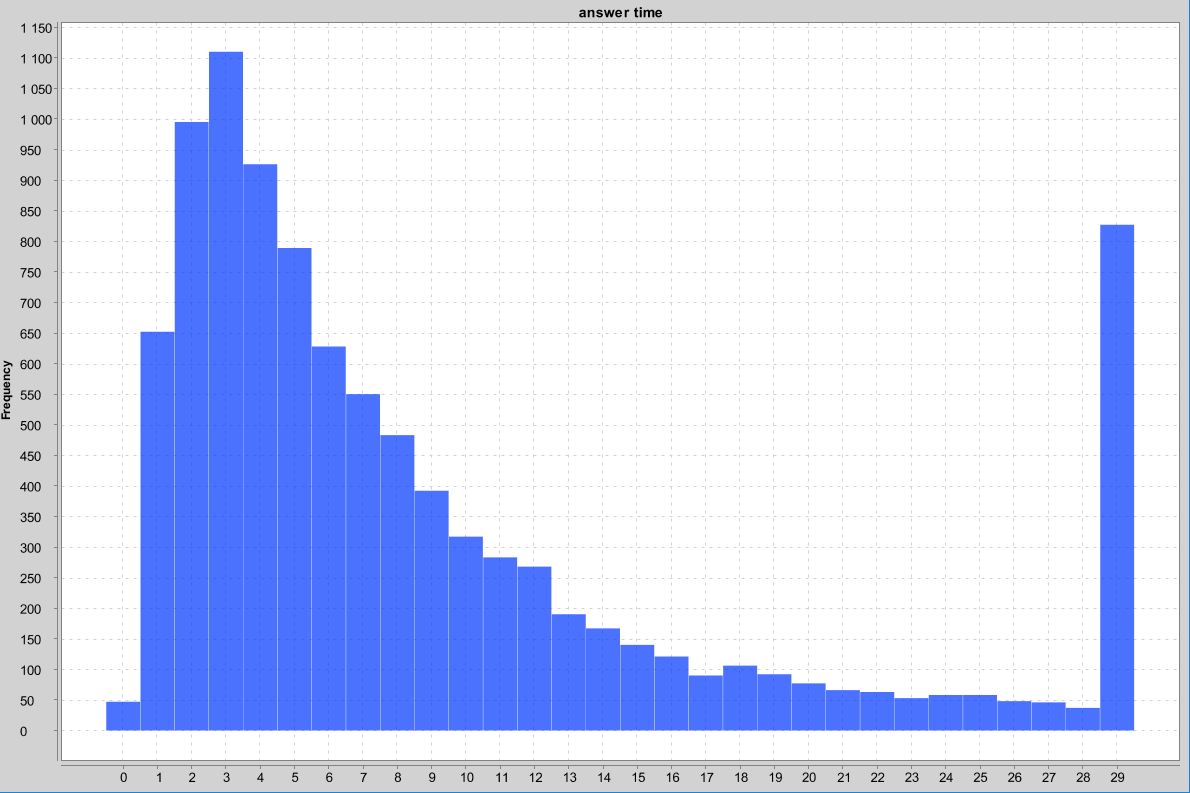
\includegraphics[scale=0.5]{answer_time.PNG}
  \caption{Время ответа на задание (в секундах). Для выбросов, портящих нормировку признака, было принято значение 30.}
  \label{fig:answer_time}
\end{figure}

\begin{figure}
  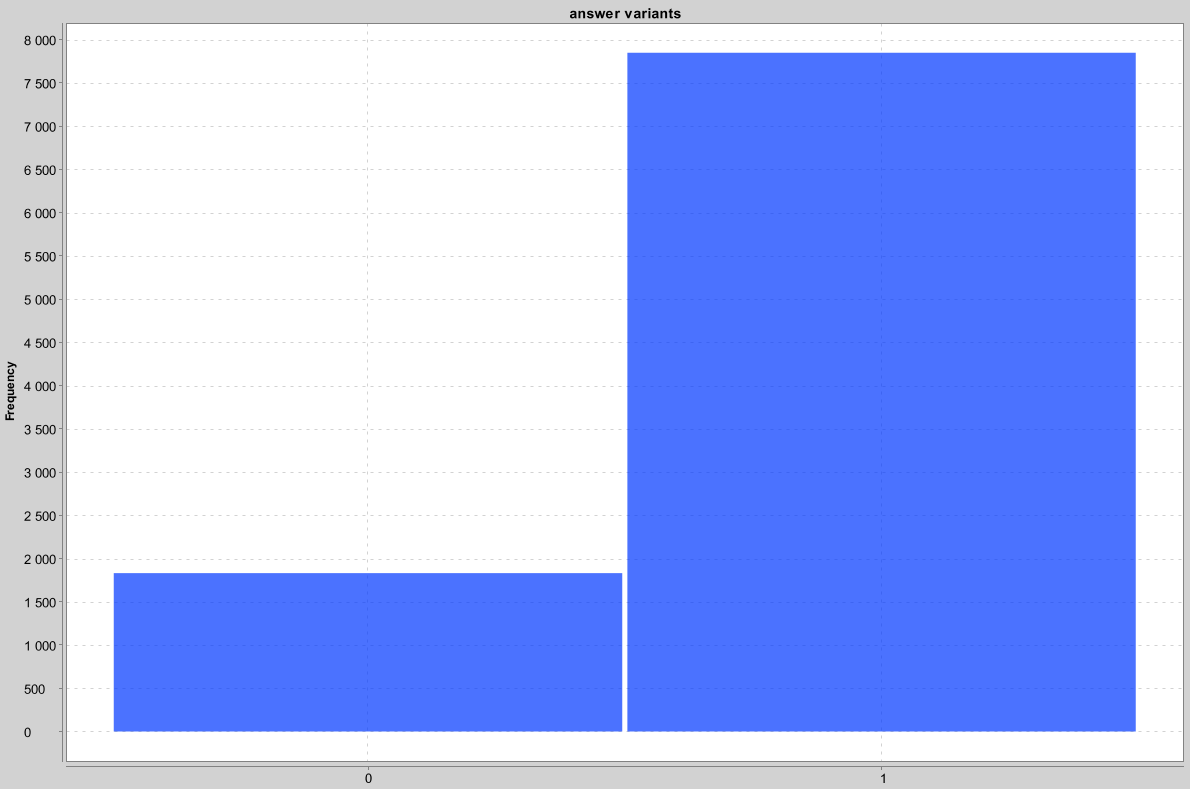
\includegraphics[scale=0.5]{answer_variants.PNG}
  \caption{Число разных выбранных вариантов ответа на задание}
  \label{fig:answer_variants}
\end{figure}

\begin{figure}
  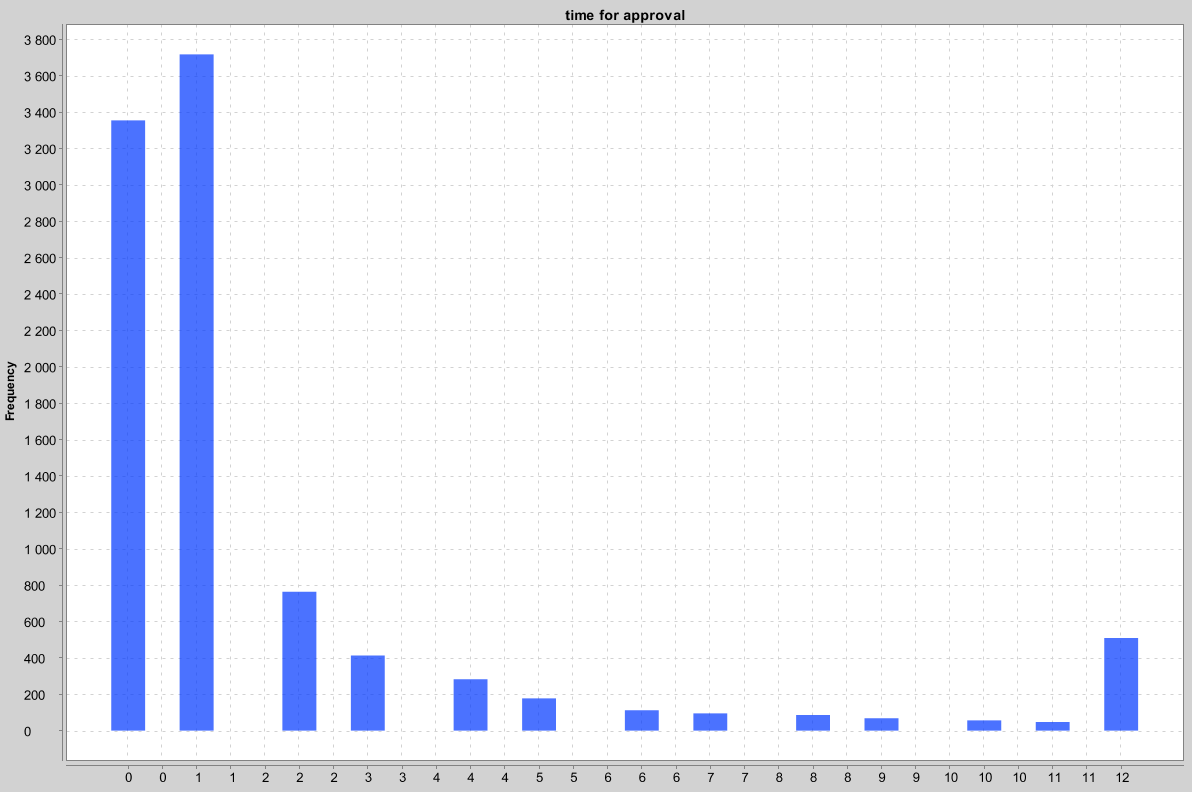
\includegraphics[scale=0.5]{time_for_approval.PNG}
  \caption{Время между подтверждением ответа и переходом к следующему заданию (в секундах). Для выбросов, портящих нормировку признака, было принято значение 12.}
  \label{fig:approval_time}
\end{figure}

\begin{figure}
  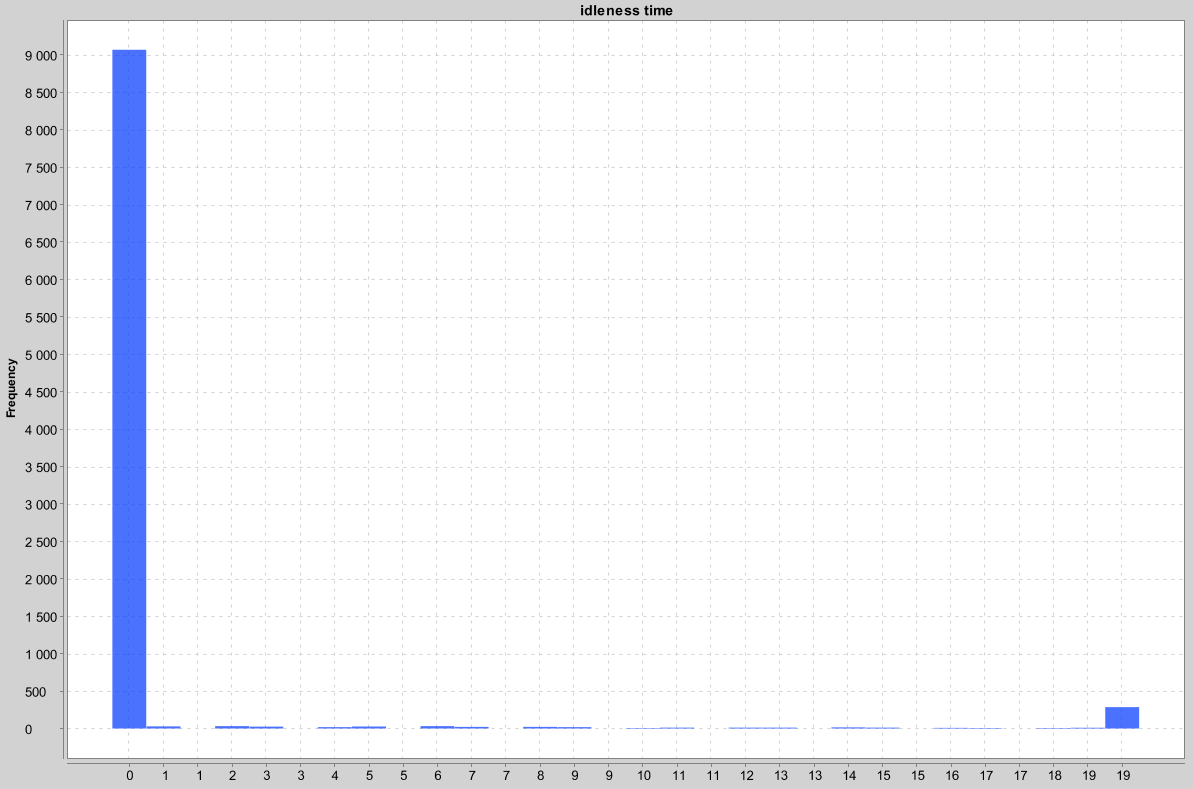
\includegraphics[scale=0.5]{idleness_time.PNG}
  \caption{Время бездействия (в секундах). Для выбросов, портящих нормировку признака, было принято значение 20.}
  \label{fig:idleness_time}
\end{figure}

\begin{figure}
  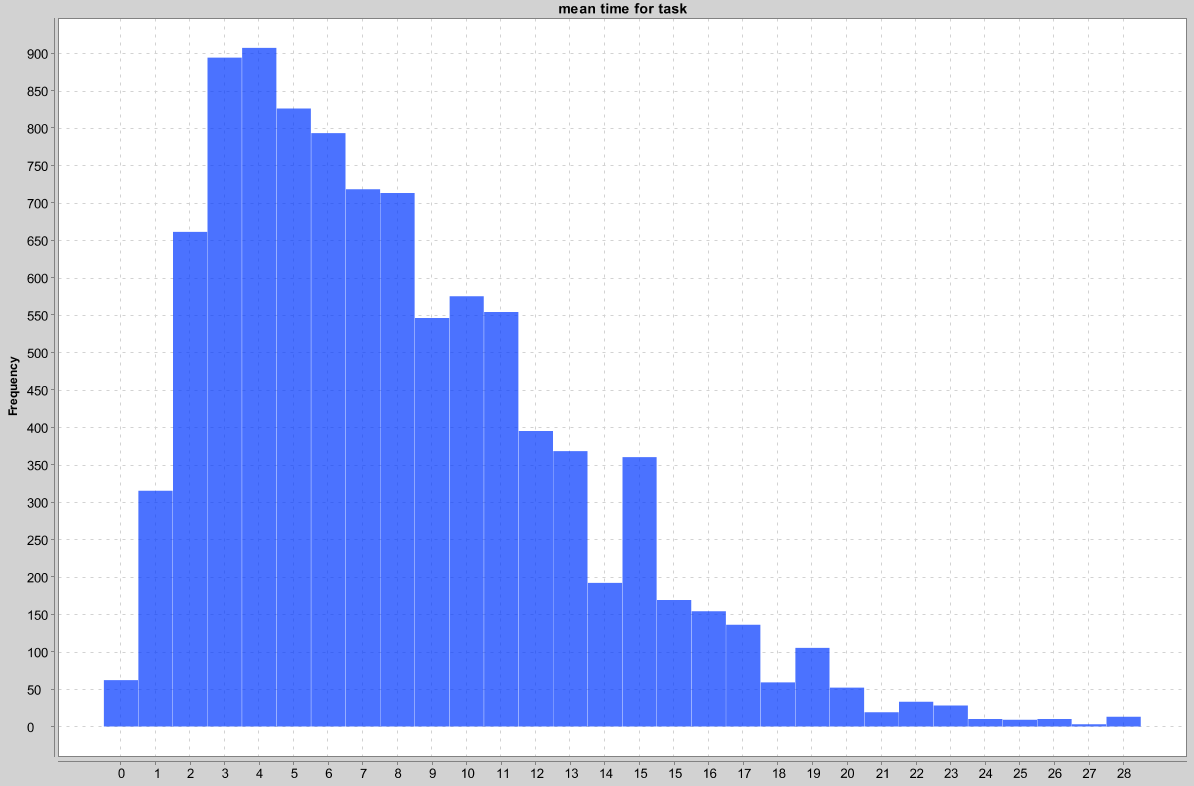
\includegraphics[scale=0.5]{mean_time_for_task.PNG}
  \caption{Среднее время ответа для задания (в секундах)}
  \label{fig:mean_time_for_task}
\end{figure}

\begin{figure}
  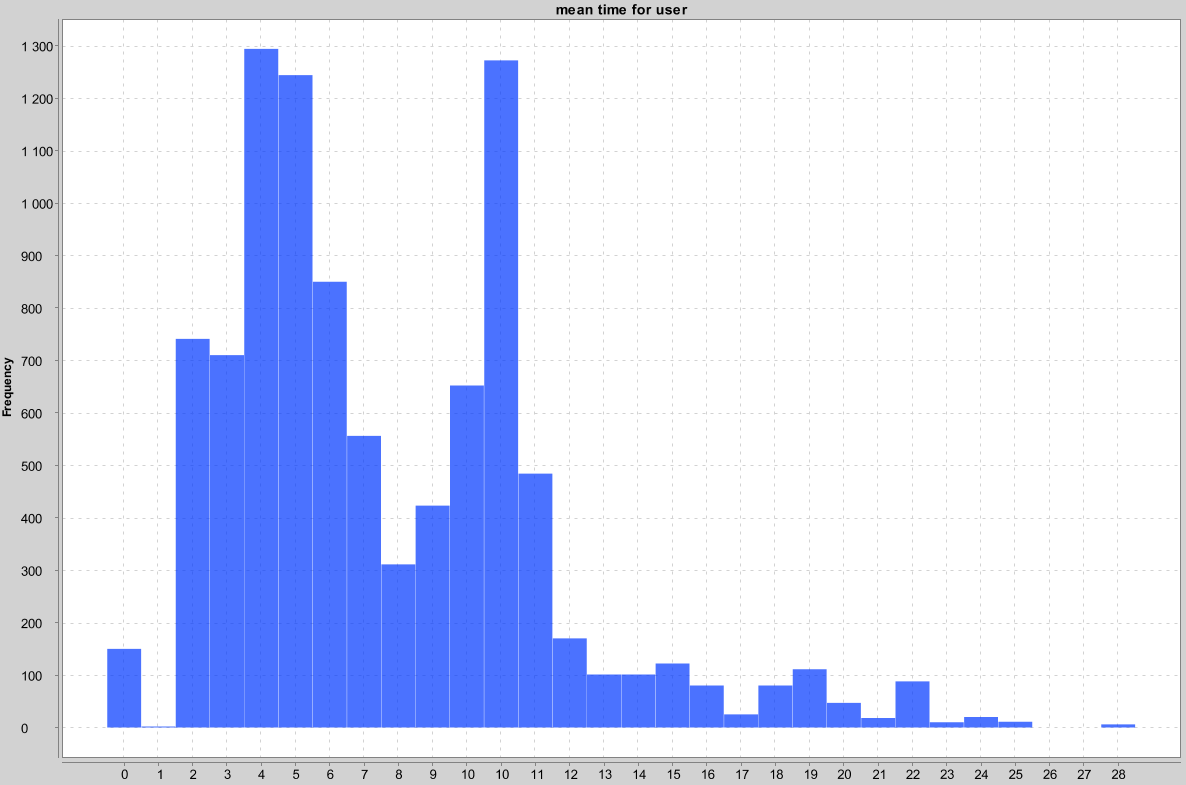
\includegraphics[scale=0.5]{mean_time_for_user.PNG}
  \caption{Среднее время ответа пользователя (в секундах)}
  \label{fig:mean_time_for_user}
\end{figure}

\begin{figure}
  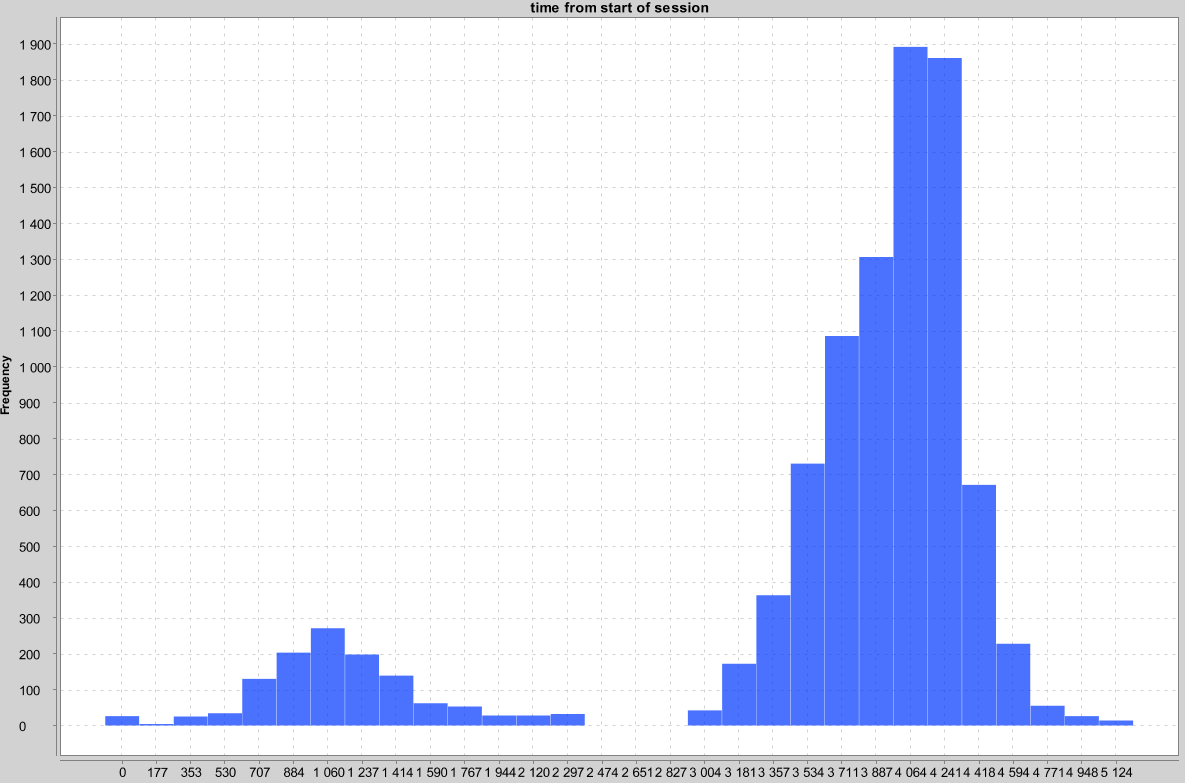
\includegraphics[scale=0.5]{time_from_start_of_session.PNG}
  \caption{Время с начала сессии (в секундах)}
  \label{fig:time_from_start_of_session}
\end{figure}

\begin{figure}
  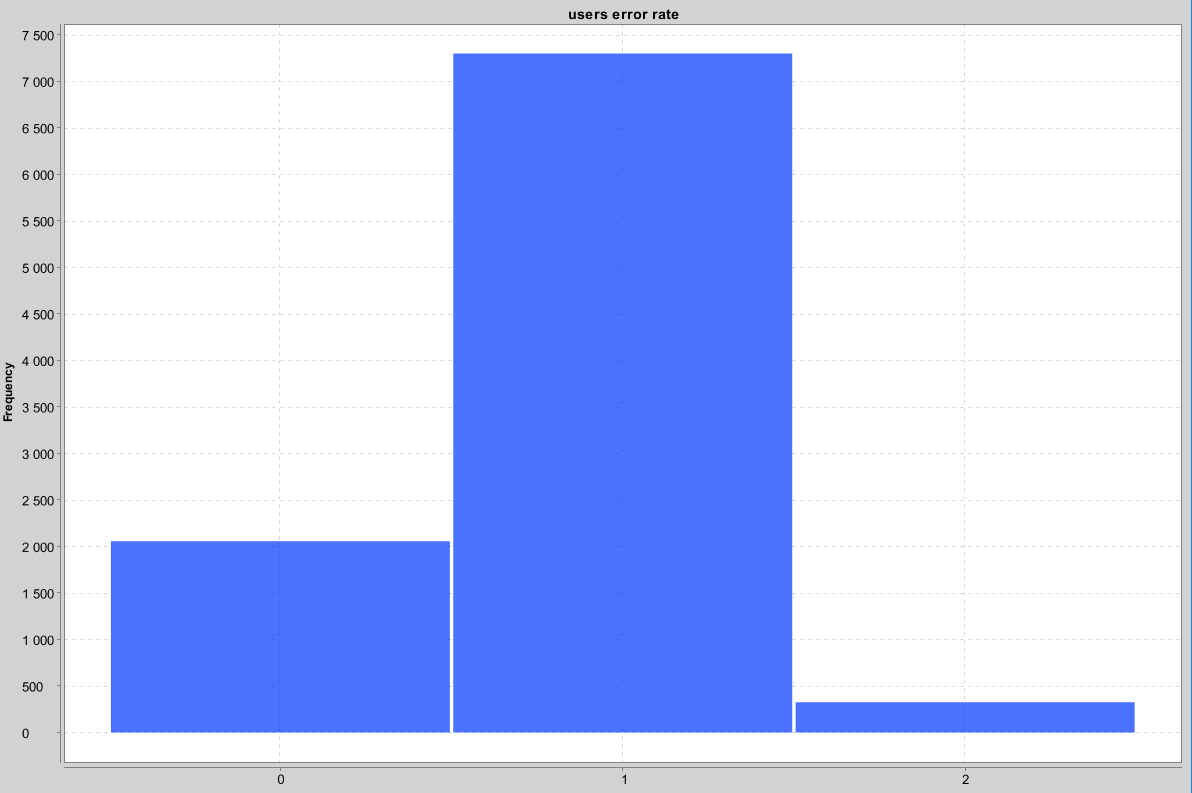
\includegraphics[scale=0.5]{users_error_rate.PNG}
  \caption{Частота ошибок пользователей. Первому столбцу со значением около 0 соответствуют компетентные исполнители, второму -- менее компетентные, допускающие больше ошибок, третьему -- спамеры.}
  \label{fig:users_error_rate}
\end{figure}

\section{Работа с данными}
Вопросы, которые задавались пользователям, были простыми. В наборе данных содержалось 396 заданий, для которых был хотя бы один неверный ответ, и 2166 заданий, для которых были только правильные ответы от пользователей. Поэтому для дальнейшего применения машинного обучения набор данных был разбит по заданиям на два множества: 
\begin{enumerate}
    \item множество заданий, для которых встречались неверные ответы;
    \item множество заданий, для которых все ответы были верными.
\end{enumerate}

Для обучения модели и получения предсказаний использовалась десятифолдовая кросс-валидация: каждое из десяти тестовых множеств содержало все ответы на примерно 40 заданий, для которых были неправильные ответы, и все ответы на примерно 217 заданий, для которых все ответы были верны. Обучающее множество было несбалансированным из-за преобладания верных ответов пользователей (в наборе данных было всего 535 ложных ответов против 9144 верных), модели было выгоднее в большинстве случаев присваивать объектам метку 1. Для решения проблемы была применена повышающая дискретизация (upsampling): в обучающее множество было равновероятно добавлено столько же объектов редкого класса, сколько было объектов класса , встречающегося часто.

Итоговая статистика по всем ответам пользователей строилась как объединение результатов для десяти тестовых множеств, полученных при кросс-валидации. 

\section{Оценка качества обученной модели}

Матрица ошибок классификации представлена в таблице \ref{confusionMatrixResult}.

\begin{table}[!h]
\caption{Матрица ошибок классификации}
\label{confusionMatrixResult}
\centering
\begin{tabularx}{\textwidth}{|*{18}{>{\centering\arraybackslash}X|}}\hline
-- & $y=1$ & $y=0$ \\\hline
$\hat{y}=1$ & 8954 (TP)  & 149 (FP)  \\\hline
$\hat{y}=0$ & 95 (FN) & 374 (TN)\\\hline
\end{tabularx}
\end{table}

По значениям из матрицы ошибок классификации были посчитаны точность (precision), полнота (recall) и $F_{1}$-мера для каждого класса и были получены их средние значения, результаты представлены в таблице \ref{fmeasure}. Значения для класса 0 (неверный ответ) ощутимо хуже, чем для класса 1, что связано с несбалансированностью набора данных.

\begin{table}[!h]
\caption{Точность, полнота, F1-мера}
\label{fmeasure}
\centering
\begin{tabularx}{\textwidth}{|*{18}{>{\centering\arraybackslash}X|}}\hline
Класс & Точность & Полнота & F1-мера \\\hline
1 (верный ответ) & 0.98 & 0.96 & 0.97\\\hline
0 (неверный ответ) & 0.8 & 0.71 & 0.75 \\\hline
Среднее значение & 0.89 & 0.84 & 0.86\\\hline
\end{tabularx}
\end{table}

Значение бинарной логистической функции потерь составило 0.07, что является хорошим показателем.

Квадратный корень из среднеквадратического отклонения между усреднённой оценкой пользователей по всем их ответам и  доли правильных ответов пользователей составил 0.07. Данное значение улучшается с ростом числа ответов пользователя, например, если взять пользователей, у которых было больше 100 ответов, и посчитать квадратный корень из среднеквадратического отклонения только для них получается 0.001. Данные значения говорят о том, что хотя классификация отдельных неверных ответов пользователей не очень хороша, судя по значению $F_{1}$ меры, средняя оценка пользователей по всем ответам даёт очень хорошие результаты.

\section{Результаты}
\subsection{Модификация метода Дэвида-Скина}

Агрегированные ответы совпали с истинными, так как вопросы были простыми, поэтому для оценки результатов использовалась вторая метрика из представленных в главе 2.

\begin{table}[!h]
\caption{Результаты с модификацией алгоритма Дэвида-Скина}
\label{resultsSkene}
\centering
\begin{tabularx}{\textwidth}{|*{18}{>{\centering\arraybackslash}X|}}\hline
-- & Качество \\\hline
Алгоритм Дэвида-Скина с оценкой исполнителей  & 0.996  \\\hline
Алгоритм Дэвида-Скина с оценкой ответов  & 0.995 \\\hline
Алгоритм Дэвида-Скина без модификаций  & 0.976 \\\hline
\end{tabularx}
\end{table}

Оценки качества агрегации на данном наборе данных для алгоритма Дэвида-Скина и его модификаций представлены в таблице \ref{resultsSkene}. Из них следует, что удалось улучшить алгоритм Дэвида-Скина на 2\%.

Исследованный набор данных содержал в основном верные ответы, поэтому немодифицированный алгоритм Дэвида-Скина выдал на нём очень высокое качество агрегированных ответов, вероятнее всего, удалось бы больше улучшить качество агрегации на наборе данных с большей долей неправильных ответов пользователей.

\subsection{Модификации голосования большинства}
Результаты для метода голосования большинства и его модификаций представлены в таблице \ref{resultsMajority}. Удалось улучшить результаты по сравнению с простым голосованием большинства на 1.7\%.
\begin{table}[!h]
\caption{Результаты с модификациями голосования большинства}
\label{resultsMajority}
\centering
\begin{tabularx}{\textwidth}{|*{18}{>{\centering\arraybackslash}X|}}\hline
-- & Качество \\\hline
Голос большинства, взвешенный поведенческими признаками и частотой ошибок из алгоритма Дэвида-Скина  & 0.956  \\\hline
Голос большинства, взвешенный поведенческими признаками  & 0.955 \\\hline
Голос большинства  & 0.939 \\\hline
\end{tabularx}
\end{table}

\subsection{Итоговые результаты}
Итоговые результаты представлены в таблице \ref{resultsSummary}.
\begin{table}[!h]
\caption{Итоговые результаты}
\label{resultsSummary}
\centering
\begin{tabularx}{\textwidth}{|*{18}{>{\centering\arraybackslash}X|}}\hline
-- & Качество \\\hline
Алгоритм Дэвида-Скина с оценкой исполнителей  & 0.996  \\\hline
Алгоритм Дэвида-Скина с оценкой ответов  & 0.995 \\\hline
Алгоритм Дэвида-Скина без модификаций  & 0.976 \\\hline
Голос большинства, взвешенный поведенческими признаками и частотой ошибок из алгоритма Дэвида-Скина  & 0.956  \\\hline
Голос большинства, взвешенный поведенческими признаками  & 0.955 \\\hline
Голос большинства  & 0.939 \\\hline
\end{tabularx}
\end{table}

\section{Важность признаков}
На рисунке \ref{fig:activity} представлен вклад признаков в ответ. Важность признаков оценена с помощью случайного леса. Лучшими признаками оказались (по убыванию значимости):
\begin{enumerate}
    \item среднее время ответа пользователя;
    \item среднее время ответа на задание;
    \item время с начала сессии;
    \item время ответа;
    \item число смен ответа.
\end{enumerate}
\begin{figure}
  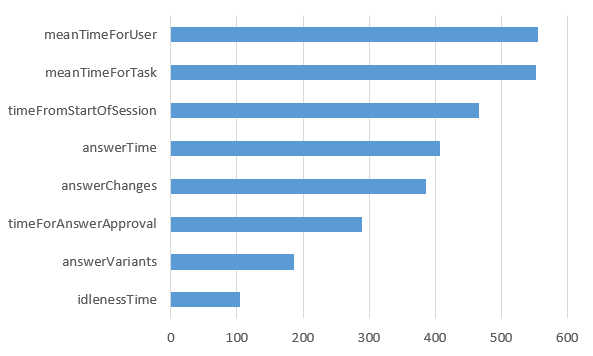
\includegraphics{features_importance.PNG}
  \caption{Вклад признаков в ответ. MeanTimeForUser -- среднее время ответа на вопрос для пользователя, meanTimeForTask -- среднее время ответа на вопрос для задания, answerChanges -- число смен ответа, timeForAnswerApproval -- время между ответом на вопрос и его подтверждением, answerVariants -- число разных вариантов ответа на вопрос, на которые пользователь наводил курсор или выбирал их, idlenessTime -- время бездействия пользователя }
  \label{fig:activity}
\end{figure}

\section{Использованные библиотеки и программное обеспечение}
Для проведения исследования и получения результатов использовалась среда разработки Intellij IDEA, язык программирования Java, система сборки Gradle. Для парсинга и записи .tsv и .csv-файлов использовалась библиотека univocity-parsers, случайный лес был взят из библиотеки smile regression, графики строились с помощью библиотеки xchart, точность, полнота, $F_{1}$-мера и матрица ошибок классификации рассчитывались с помощью библиотеки org.apache.commons.

\chapterconclusion
В главе 3 были описаны исходные данные для эксперимента и способ их обработки. Были представлены результаты сравнения модификации алгоритма Дэвида-Скина с его же версий без модификации, удалось улучшить качество агрегации ответов. Был составлен список наиболее удачно подобранных признаков, внёсших наибольший вклад в результат. Были описаны модификации метода голосования большинства, дающие лучший результат, чем простой метод голосования большинства. Была приведена оценка качества обученной модели машинного обучения. Были описаны использованные библиотеки и программное обеспечение.

%% Макрос для заключения. Совместим со старым стилевиком.
\startconclusionpage
В работе предложен способ модификации широко использующегося при агрегации ответов в краудсорсинге и хорошо себя зарекомендовавшего алгоритма Дэвида-Скина. Предложенный метод учитывает поведение пользователей, что позволяет бороться с такими проблемами как падение концентрации пользователя с течением времени, сомнения в ответе.

Полученный метод можно внедрять в краудсорсинговые платформы и получать более качественные результаты.

\printmainbibliography

%% После этой команды chapter будет генерировать приложения, нумерованные русскими буквами.
%% \startappendices из старого стилевика будет делать то же самое
\appendix

%%\chapter{Пример приложения}\label{sec:app:1}


%%\chapter{Пример огромного листинга}

                

\end{document}
